\section{AM Convencional (DSB-LC)}

\begin{frame}{AM Convencional (DSB-LC): A Ideia}

\textbf{Problema do DSB-SC:} Requer sincronização perfeita do oscilador local

\vspace{0.3cm}

\textbf{Pergunta:} E se transmitirmos junto a portadora?

\vspace{0.3cm}

\begin{center}
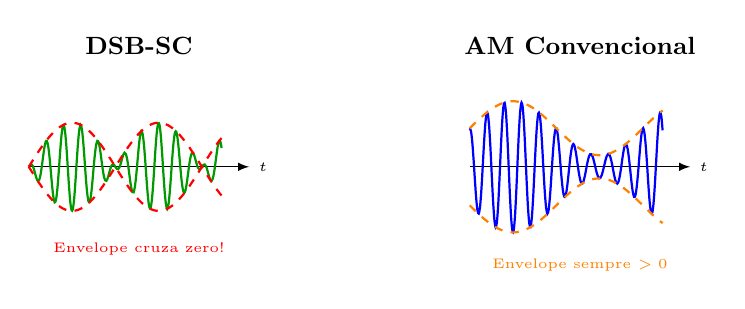
\begin{tikzpicture}[>=latex, scale=0.7]
% DSB-SC
\begin{scope}[xshift=-4cm]
\node[font=\small\bfseries] at (2,2.2) {DSB-SC};
\draw[->] (0,0) -- (4,0) node[right, font=\tiny] {$t$};
\draw[thick, green!60!black, smooth] plot[domain=0:3.5, samples=150] (\x, {0.8*sin(2*\x r)*cos(20*\x r)});
\draw[thick, dashed, red, smooth] plot[domain=0:3.5, samples=80] (\x, {0.8*sin(2*\x r)});
\draw[thick, dashed, red, smooth] plot[domain=0:3.5, samples=80] (\x, {-0.8*sin(2*\x r)});
\node[below, font=\tiny, red] at (2,-1.2) {Envelope cruza zero!};
\end{scope}

% AM Convencional
\begin{scope}[xshift=4cm]
\node[font=\small\bfseries] at (2,2.2) {AM Convencional};
\draw[->] (0,0) -- (4,0) node[right, font=\tiny] {$t$};
\draw[thick, blue, smooth] plot[domain=0:3.5, samples=150] (\x, {(1+0.7*sin(2*\x r))*0.7*cos(20*\x r)});
\draw[thick, dashed, orange, smooth] plot[domain=0:3.5, samples=80] (\x, {(1+0.7*sin(2*\x r))*0.7});
\draw[thick, dashed, orange, smooth] plot[domain=0:3.5, samples=80] (\x, {-(1+0.7*sin(2*\x r))*0.7});
\node[below, font=\tiny, orange] at (2,-1.5) {Envelope sempre $> 0$};
\end{scope}
\end{tikzpicture}
\end{center}

\textbf{AM Convencional:} Adiciona portadora ao DSB-SC $\rightarrow$ envelope sempre positivo

$\rightarrow$ Permite demodulação com \textbf{detector de envelope} (simples e barato!)

\end{frame}

% ============================================

\begin{frame}{Definição: AM Convencional (DSB-LC)}

\begin{block}{Definição}
\vspace{-0.3cm}
\[
s(t) = A_c[1 + k_a m(t)] \cos(2\pi f_c t)
\]
\end{block}

\onslide<2->{
\textbf{Decomposição:}
\[
s(t) = \underbrace{A_c \cos(2\pi f_c t)}_{\text{portadora}} + \underbrace{A_c k_a m(t) \cos(2\pi f_c t)}_{\text{DSB-SC}}
\]
}

\onslide<3->{
\begin{center}
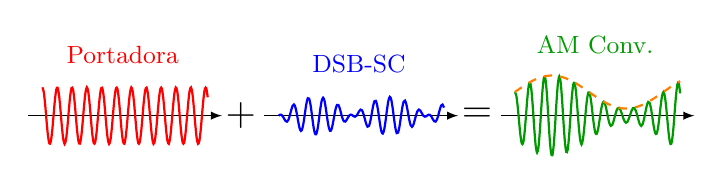
\begin{tikzpicture}[>=latex, scale=0.6]
% Portadora pura
\begin{scope}[xshift=-5cm]
\draw[->] (-0.3,0) -- (3.8,0);
\draw[thick, red, smooth] plot[domain=0:3.5, samples=120]
  (\x, {0.6*cos(20*\x r)});
\node[above, font=\small, red] at (1.7,0.9) {Portadora};
\end{scope}
% Sinal +
\node[font=\Large] at (-0.8,0) {$+$};
% DSB-SC
\begin{scope}[xshift=0cm]
\draw[->] (-0.3,0) -- (3.8,0);
\draw[thick, blue, smooth] plot[domain=0:3.5, samples=120]
  (\x, {0.4*sin(2*\x r)*cos(20*\x r)});
\node[above, font=\small, blue] at (1.7,0.7) {DSB-SC};
\end{scope}
% Sinal =
\node[font=\Large] at (4.2,0) {$=$};
% AM
\begin{scope}[xshift=5cm]
\draw[->] (-0.3,0) -- (3.8,0);
\draw[thick, green!60!black, smooth] plot[domain=0:3.5, samples=120]
  (\x, {(1+0.7*sin(2*\x r))*0.5*cos(20*\x r)});
\draw[thick, dashed, orange, smooth] plot[domain=0:3.5, samples=60]
  (\x, {(1+0.7*sin(2*\x r))*0.5});
\node[above, font=\small, green!60!black] at (1.7,1.1) {AM Conv.};
\end{scope}
\end{tikzpicture}
\end{center}
}

\onslide<4->{
\textbf{Preço:} Gastar potência transmitindo portadora (sem informação!)

\textbf{Ganho:} Receptor com simples \textbf{detector de envelope}
}

\end{frame}

% ============================================

\begin{frame}{Índice de Modulação $\mu$}

\textbf{Normalizando} $m(t)$ tal que $\max|m(t)| = 1$:

\textbf{Índice de modulação:} $\mu = k_a$

\[
\boxed{s(t) = A_c[1 + \mu m_n(t)] \cos(2\pi f_c t)}
\]

\textbf{Envelope:} $A(t) = A_c[1 + \mu m_n(t)]$

\vspace{0.3cm}

\begin{columns}[T]
\begin{column}{0.45\textwidth}
\textbf{Valores de $\mu$:}
\begin{itemize}
\item $\mu = 0$: portadora pura
\item $0 < \mu < 1$: operação normal
\item $\mu = 1$: modulação 100\%
\item $\mu > 1$: \textbf{supermodulação!}
\end{itemize}
\end{column}
\begin{column}{0.52\textwidth}
\begin{center}
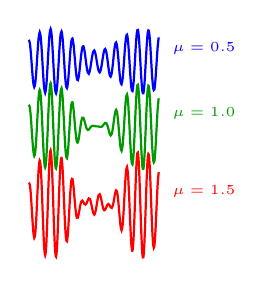
\begin{tikzpicture}[>=latex, scale=0.55]
% mu = 0.5
\begin{scope}[yshift=1.5cm]
\draw[thick, blue, smooth] plot[domain=0:3, samples=120] (\x, {(1+0.5*sin(3*\x r))*0.5*cos(25*\x r)});
\node[right, font=\tiny, blue] at (3.1,0.3) {$\mu = 0.5$};
\end{scope}
% mu = 1.0
\begin{scope}[yshift=0cm]
\draw[thick, green!60!black, smooth] plot[domain=0:3, samples=120] (\x, {(1+1.0*sin(3*\x r))*0.5*cos(25*\x r)});
\node[right, font=\tiny, green!60!black] at (3.1,0.3) {$\mu = 1.0$};
\end{scope}
% mu = 1.5
\begin{scope}[yshift=-1.8cm]
\draw[thick, red, smooth] plot[domain=0:3, samples=120] (\x, {(1+1.5*sin(3*\x r))*0.5*cos(25*\x r)});
\node[right, font=\tiny, red] at (3.1,0.3) {$\mu = 1.5$};
\end{scope}
\end{tikzpicture}
\end{center}
\end{column}
\end{columns}

\end{frame}

% ============================================

\begin{frame}{Visualização AM: $\mu = 0.5$ e $\mu = 1.0$}

\begin{center}
\includegraphics[width=\figFull, height=0.7\textheight, keepaspectratio, trim=0 235bp 0 0, clip]{figures/cap4/am_conventional.pdf}
\end{center}

\vspace{-2mm}
\textbf{$\mu = 0.5$:} Envelope sempre positivo. \quad \textbf{$\mu = 1.0$:} Envelope toca zero.

\end{frame}

% ============================================

\begin{frame}{Supermodulação: Sinal no Tempo}

\begin{center}
\includegraphics[width=\figFull]{figures/cap4/supermod_tempo.pdf}
\end{center}

\vspace{-0.2cm}
Para $\mu > 1$, o envelope $1 + \mu\,m(t)$ fica negativo $\rightarrow$ a portadora \textbf{inverte a fase} (salto de $180°$).

\end{frame}

% ============================================

\begin{frame}{Supermodulação: Distorção no Detector de Envelope}

\begin{center}
\includegraphics[width=\figFull]{figures/cap4/supermod_detector.pdf}
\end{center}

\vspace{-0.2cm}
O detector de envelope extrai $|1 + \mu\,m(t)|$: as partes negativas ``rebatem'' para cima $\rightarrow$ \textbf{distorção}.

\end{frame}

% ============================================

\begin{frame}{Supermodulação: Espectro Transmitido}

\begin{center}
\includegraphics[width=\figFull]{figures/cap4/supermod_espectro_rf.pdf}
\end{center}

\vspace{-0.2cm}
O espectro transmitido tem as \textbf{mesmas componentes} ($f_c$ e $f_c \pm f_m$) --- o problema não está aqui!

\end{frame}

% ============================================

\begin{frame}{Supermodulação: Distorção na Detecção}

\begin{center}
\includegraphics[width=\figFull]{figures/cap4/supermod_espectro_bb.pdf}
\end{center}

\vspace{-0.2cm}
A distorção surge na \textbf{detecção}: $|1+\mu\,m(t)|$ é não-linear $\rightarrow$ gera harmônicas $2f_m, 3f_m, \ldots$ que \textbf{não existiam} em $m(t)$.

\end{frame}

% ============================================

\begin{frame}{Supermodulação: Por que Evitar?}

\textbf{Condição de supermodulação:} $\mu > 1$ ou $|k_a m(t)| > 1$

\textbf{Problema:}
\[
1 + k_a m(t) < 0 \quad \text{para alguns valores de } t
\]

Envelope torna-se negativo $\rightarrow$ inversão de fase $\rightarrow$ distorção

\vspace{0.3cm}

\textbf{Consequências:}
\begin{itemize}
\item Detector de envelope produz saída distorcida
\item Espectro contém componentes espúrias
\item Ineficiência de potência
\item \textbf{Deve ser evitada!}
\end{itemize}

\vspace{0.3cm}

\textbf{Solução:} Controle automático de ganho (AGC) no transmissor

\end{frame}

% ============================================

\begin{frame}{Espectro do AM Convencional}

\only<1>{
\[
s(t) = \underbrace{A_c \cos(2\pi f_c t)}_{\text{portadora}} + \underbrace{A_c k_a m(t) \cos(2\pi f_c t)}_{\text{bandas laterais}}
\]

\textbf{Transformada de Fourier:}
\[
S(f) = \underbrace{\frac{A_c}{2}[\delta(f\!-\!f_c) + \delta(f\!+\!f_c)]}_{\text{portadora}} + \underbrace{\frac{A_c k_a}{2}[M(f\!-\!f_c) + M(f\!+\!f_c)]}_{\text{bandas laterais}}
\]
}

\only<2>{
\begin{center}
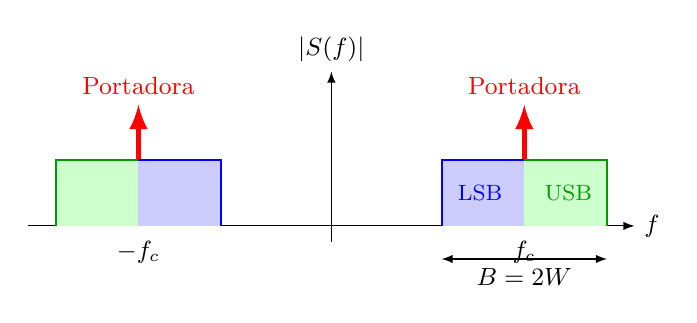
\begin{tikzpicture}[>=latex, scale=0.7]
\draw[->] (-5.5,0) -- (5.5,0) node[right, font=\small] {$f$};
\draw[->] (0,-0.3) -- (0,2.8) node[above, font=\small] {$|S(f)|$};
% Portadora (impulsos)
\draw[thick, red, ->, line width=2pt] (-3.5,0) -- (-3.5,2.2);
\draw[thick, red, ->, line width=2pt] (3.5,0) -- (3.5,2.2);
\node[above, font=\small, red] at (3.5,2.2) {Portadora};
\node[above, font=\small, red] at (-3.5,2.2) {Portadora};
% Bandas laterais
\fill[blue!20] (2,0) -- (2,1.2) -- (3.5,1.2) -- (3.5,0) -- cycle;
\fill[green!20] (3.5,0) -- (3.5,1.2) -- (5,1.2) -- (5,0) -- cycle;
\draw[thick, blue] (2,0) -- (2,1.2) -- (3.5,1.2);
\draw[thick, green!60!black] (3.5,1.2) -- (5,1.2) -- (5,0);
\fill[green!20] (-5,0) -- (-5,1.2) -- (-3.5,1.2) -- (-3.5,0) -- cycle;
\fill[blue!20] (-3.5,0) -- (-3.5,1.2) -- (-2,1.2) -- (-2,0) -- cycle;
\draw[thick, green!60!black] (-5,0) -- (-5,1.2) -- (-3.5,1.2);
\draw[thick, blue] (-3.5,1.2) -- (-2,1.2) -- (-2,0);
% Labels
\node[below, font=\small] at (3.5,-0.1) {$f_c$};
\node[below, font=\small] at (-3.5,-0.1) {$-f_c$};
\node[font=\footnotesize, blue] at (2.7,0.6) {LSB};
\node[font=\footnotesize, green!60!black] at (4.3,0.6) {USB};
% Banda
\draw[<->] (2,-0.6) -- (5,-0.6) node[midway, below, font=\small] {$B = 2W$};
\end{tikzpicture}
\end{center}

\vspace{0.2cm}

\textbf{vs.\ DSB-SC:} Mesma largura de banda $B = 2W$, mas com \textbf{portadora} dominante em $\pm f_c$
}

\end{frame}

% ============================================

\begin{frame}{Potência e Eficiência do AM Convencional}

\only<1>{
\textbf{Potência total} (para $\langle m(t)\rangle = 0$):
\[
P_s = \underbrace{\frac{A_c^2}{2}}_{P_c \text{ (portadora)}} + \underbrace{\frac{A_c^2 k_a^2 P_m}{2}}_{P_{sb} \text{ (bandas laterais)}}
\]

\textbf{Eficiência:} Fração da potência que carrega informação
\[
\boxed{\eta = \frac{P_{sb}}{P_s} = \frac{k_a^2 P_m}{1 + k_a^2 P_m}}
\]

Para tom único ($P_m = 1/2$): $\eta = \dfrac{\mu^2}{2 + \mu^2}$
}

\only<2>{
\begin{columns}[T]
\begin{column}{0.48\textwidth}
\begin{center}
\includegraphics[width=\textwidth]{figures/cap4/am_efficiency.pdf}
\end{center}
\end{column}
\begin{column}{0.50\textwidth}

\textbf{Eficiências típicas:}

\vspace{0.2cm}

\begin{tabular}{c c l}
$\mu$ & $\eta$ & \\
\hline
$0.3$ & $4.3\%$ & Muito baixa \\
$0.5$ & $11\%$ & Baixa \\
$0.8$ & $24\%$ & Típica \\
$1.0$ & $33\%$ & \textbf{Máxima!} \\
\end{tabular}

\vspace{0.3cm}

Mesmo no melhor caso ($\mu = 1$), \textbf{2/3 da potência é desperdiçada} na portadora!

\vspace{0.2cm}

\textbf{Compensa pela simplicidade} do receptor
\end{column}
\end{columns}
}

\end{frame}

% ============================================

\begin{frame}{Exemplo: Estação de Rádio AM}

\begin{block}{Enunciado}
Uma estação de rádio AM transmite um tom de áudio $m(t) = \cos(2\pi \cdot 5000\, t)$
com portadora $f_c = 1\,\text{MHz}$, $A_c = 100\,\text{V}$ e índice $\mu = 0.8$.
\end{block}

\onslide<2->{
\textbf{Determine:}
\begin{enumerate}
\item O sinal AM transmitido e suas componentes espectrais
\item A potência na portadora, nas bandas laterais e a eficiência
\item Compare com DSB-SC nas mesmas condições
\end{enumerate}
}

\onslide<3->{
\vspace{0.3cm}
\begin{center}
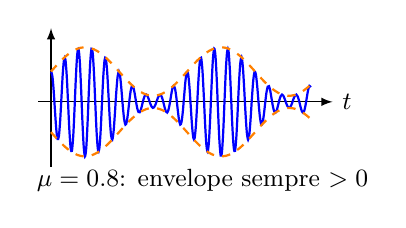
\begin{tikzpicture}[>=latex, scale=0.55]
% Sinal AM no tempo
\draw[->] (-0.3,0) -- (6.5,0) node[right, font=\small] {$t$};
\draw[->] (0,-1.5) -- (0,1.7);
\draw[thick, blue, smooth] plot[domain=0:6, samples=200]
  (\x, {(1+0.8*sin(2*\x r))*0.7*cos(20*\x r)});
\draw[thick, dashed, orange, smooth] plot[domain=0:6, samples=80]
  (\x, {(1+0.8*sin(2*\x r))*0.7});
\draw[thick, dashed, orange, smooth] plot[domain=0:6, samples=80]
  (\x, {-(1+0.8*sin(2*\x r))*0.7});
\node[font=\small] at (3.5,-1.8) {$\mu = 0.8$: envelope sempre $> 0$};
\end{tikzpicture}
\end{center}
}

\end{frame}

% ============================================

\begin{frame}{Resolução: Estação de Rádio AM}

\only<1>{
\textbf{Passo 1: Expressão do sinal AM}

\[
s(t) = 100[1 + 0.8\cos(2\pi \cdot 5000\, t)] \cos(2\pi \cdot 10^6\, t)
\]

Expandindo usando $\cos A \cos B = \frac{1}{2}[\cos(A-B) + \cos(A+B)]$:

\vspace{-0.2cm}

\begin{align*}
s(t) &= \underbrace{100\cos(2\pi \cdot 10^6 t)}_{\text{portadora: amplitude } 100}\\[4pt]
&+ \underbrace{40\cos(2\pi \cdot 995000\, t)}_{\text{LSB: amplitude } 40}
+ \underbrace{40\cos(2\pi \cdot 1005000\, t)}_{\text{USB: amplitude } 40}
\end{align*}

\textbf{Três componentes:} portadora em $f_c$ + duas bandas laterais em $f_c \pm f_m$
}

\only<2>{
\textbf{Passo 1 (cont.): Espectro}

\begin{center}
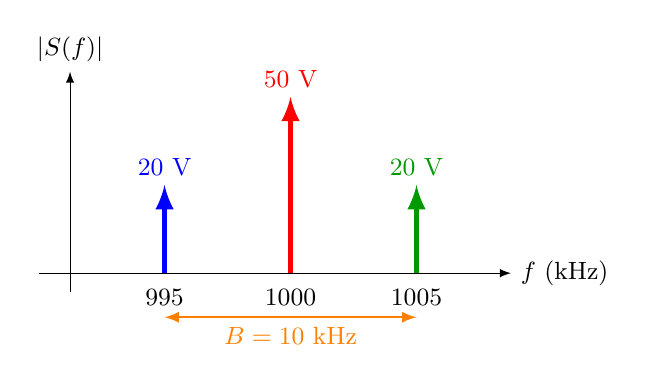
\begin{tikzpicture}[>=latex, scale=0.8]
\draw[->] (-0.5,0) -- (7,0) node[right, font=\small] {$f$ (kHz)};
\draw[->] (0,-0.3) -- (0,3.2) node[above, font=\small] {$|S(f)|$};
% Portadora
\draw[thick, red, ->, line width=2pt] (3.5,0) -- (3.5,2.8);
\node[above, font=\small, red] at (3.5,2.8) {$50$ V};
\node[below, font=\small] at (3.5,-0.1) {$1000$};
% LSB
\draw[thick, blue, ->, line width=2pt] (1.5,0) -- (1.5,1.4);
\node[above, font=\small, blue] at (1.5,1.4) {$20$ V};
\node[below, font=\small] at (1.5,-0.1) {$995$};
% USB
\draw[thick, green!60!black, ->, line width=2pt] (5.5,0) -- (5.5,1.4);
\node[above, font=\small, green!60!black] at (5.5,1.4) {$20$ V};
\node[below, font=\small] at (5.5,-0.1) {$1005$};
% Banda
\draw[<->, thick, orange] (1.5,-0.7) -- (5.5,-0.7) node[midway, below, font=\small] {$B = 10$ kHz};
\end{tikzpicture}
\end{center}

Portadora \textbf{domina} o espectro ($50$ V vs.\ $20$ V nas bandas laterais)
}

\only<3>{
\textbf{Passo 2: Potências e eficiência}

\vspace{0.2cm}

\begin{columns}[T]
\begin{column}{0.55\textwidth}
\textbf{Potência da portadora:}
\[
P_c = \frac{A_c^2}{2} = \frac{100^2}{2} = 5000\,\text{W}
\]

\textbf{Potência nas bandas laterais:}
\[
P_{sb} = \frac{\mu^2}{2} P_c = \frac{0.64}{2} \times 5000 = 1600\,\text{W}
\]

\textbf{Potência total:}
\[
P_s = 5000 + 1600 = \boxed{6600\,\text{W}}
\]

\textbf{Eficiência:}
\[
\eta = \frac{1600}{6600} = \boxed{24.2\%}
\]
\end{column}
\begin{column}{0.43\textwidth}
\begin{center}
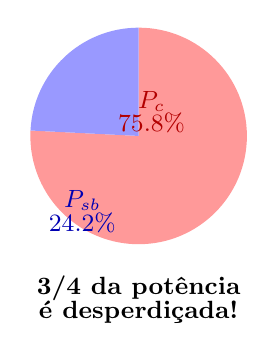
\begin{tikzpicture}[scale=0.55]
% Gráfico de pizza simplificado
\fill[red!40] (0,0) -- (0,2.5) arc (90:90-360*0.758:2.5) -- cycle;
\fill[blue!40] (0,0) -- (90-360*0.758:2.5) arc (90-360*0.758:90-360:2.5) -- cycle;
\node[font=\small, red!70!black] at (0.3,0.8) {$P_c$};
\node[font=\small, red!70!black] at (0.3,0.3) {75.8\%};
\node[font=\small, blue!70!black] at (-1.3,-1.5) {$P_{sb}$};
\node[font=\small, blue!70!black] at (-1.3,-2) {24.2\%};
\node[below, font=\small\bfseries] at (0,-3) {3/4 da potência};
\node[below, font=\small\bfseries] at (0,-3.6) {é desperdiçada!};
\end{tikzpicture}
\end{center}
\end{column}
\end{columns}
}

\only<3>{
\textbf{Passo 3: Comparação com DSB-SC}

\vspace{0.3cm}

\begin{center}
\begin{tabular}{l c c}
\textbf{Parâmetro} & \textbf{AM Conv.} & \textbf{DSB-SC} \\
\hline
Potência total & 6600 W & 2500 W \\
Potência útil & 1600 W & 2500 W \\
Eficiência $\eta$ & 24.2\% & 100\% \\
Largura de banda & 10 kHz & 10 kHz \\
Receptor & Envelope & Coerente \\
\end{tabular}
\end{center}

\vspace{0.3cm}

\begin{center}
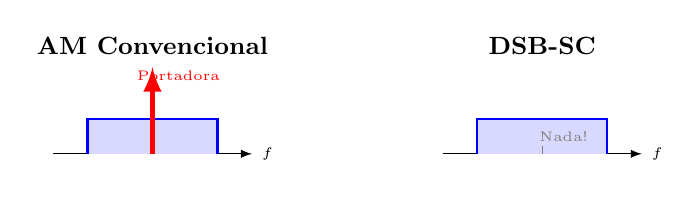
\begin{tikzpicture}[>=latex, scale=0.55]
% AM Conv espectro
\begin{scope}[xshift=-4.5cm]
\node[font=\small\bfseries] at (2,2.5) {AM Convencional};
\draw[->] (-0.3,0) -- (4.3,0) node[right, font=\tiny] {$f$};
\fill[blue!15] (0.5,0) -- (0.5,0.8) -- (2,0.8) -- (2,0) -- cycle;
\fill[blue!15] (2,0) -- (2,0.8) -- (3.5,0.8) -- (3.5,0) -- cycle;
\draw[thick, blue] (0.5,0) -- (0.5,0.8) -- (3.5,0.8) -- (3.5,0);
\draw[thick, red, ->, line width=2pt] (2,0) -- (2,2);
\node[font=\tiny, red] at (2.6,1.8) {Portadora};
\end{scope}
% DSB-SC espectro
\begin{scope}[xshift=4.5cm]
\node[font=\small\bfseries] at (2,2.5) {DSB-SC};
\draw[->] (-0.3,0) -- (4.3,0) node[right, font=\tiny] {$f$};
\fill[blue!15] (0.5,0) -- (0.5,0.8) -- (2,0.8) -- (2,0) -- cycle;
\fill[blue!15] (2,0) -- (2,0.8) -- (3.5,0.8) -- (3.5,0) -- cycle;
\draw[thick, blue] (0.5,0) -- (0.5,0.8) -- (3.5,0.8) -- (3.5,0);
\draw[dashed, gray] (2,0) -- (2,0.5);
\node[font=\tiny, gray] at (2.5,0.4) {Nada!};
\end{scope}
\end{tikzpicture}
\end{center}

\textbf{AM broadcast escolhe simplicidade:} milhões de receptores baratos vs.\ poucos transmissores caros
}

\end{frame}

% ============================================

\begin{frame}{Detector de Envelope}

\only<1>{
\textbf{Vantagem do AM convencional:} Demodulação sem oscilador local!

\vspace{0.3cm}

\begin{center}
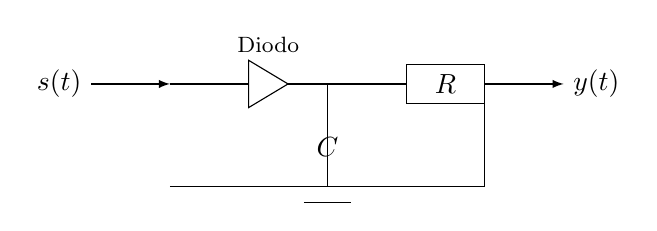
\begin{tikzpicture}[>=latex, scale=1.0]
% Diodo
\draw (0,0) -- (1,0);
\draw[fill=white] (1,-0.3) -- (1,0.3) -- (1.5,0) -- cycle;
\draw (1.5,0) -- (2,0);
% Capacitor
\draw (2,0) -- (2,-1.3);
\draw (1.7,-1.3) -- (2.3,-1.3);
\draw (1.7,-1.5) -- (2.3,-1.5);
% Resistor
\draw (2,0) -- (3,0);
\draw (3,-0.25) rectangle (4,0.25);
\node at (3.5,0) {$R$};
\draw (4,0) -- (4,-1.3);
% Terra
\draw (0,-1.3) -- (4,-1.3);
% Entrada/Saída
\draw[<-] (0,0) -- (-1,0) node[left] {$s(t)$};
\draw[->] (4,0) -- (5,0) node[right] {$y(t)$};
% Labels
\node at (2,-0.8) {$C$};
\node at (1.25,0.5) {\footnotesize Diodo};
\end{tikzpicture}
\end{center}

\vspace{0.2cm}

\textbf{Condição:} $\dfrac{1}{f_c} \ll RC \ll \dfrac{1}{W}$

Razão do sucesso do AM broadcast: receptor de 1 componente!
}

\only<2>{
\textbf{Como funciona passo a passo:}

\begin{center}
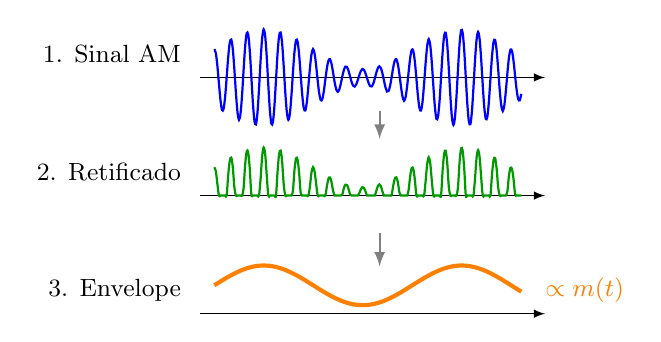
\begin{tikzpicture}[>=latex, scale=0.6]
% Sinal AM original
\begin{scope}[yshift=2.5cm]
\node[left, font=\small] at (-0.5,0.5) {1. Sinal AM};
\draw[->] (-0.3,0) -- (7,0);
\draw[thick, blue, smooth] plot[domain=0:6.5, samples=200]
  (\x, {(1+0.7*sin(1.5*\x r))*0.6*cos(18*\x r)});
\end{scope}
% Após diodo (retificado)
\begin{scope}[yshift=0cm]
\node[left, font=\small] at (-0.5,0.5) {2. Retificado};
\draw[->] (-0.3,0) -- (7,0);
\draw[thick, green!60!black, smooth] plot[domain=0:6.5, samples=200]
  (\x, {max(0, (1+0.7*sin(1.5*\x r))*0.6*cos(18*\x r))});
\end{scope}
% Após RC (envelope)
\begin{scope}[yshift=-2.5cm]
\node[left, font=\small] at (-0.5,0.5) {3. Envelope};
\draw[->] (-0.3,0) -- (7,0);
\draw[thick, orange, smooth, line width=1.5pt] plot[domain=0:6.5, samples=80]
  (\x, {(1+0.7*sin(1.5*\x r))*0.6});
\node[right, font=\small, orange] at (6.8,0.5) {$\propto m(t)$};
\end{scope}
% Setas
\draw[->, thick, gray] (3.5,1.8) -- (3.5,1.2);
\draw[->, thick, gray] (3.5,-0.8) -- (3.5,-1.5);
\end{tikzpicture}
\end{center}
}

\end{frame}

% ============================================

\begin{frame}{Resumo: DSB-SC vs. AM Convencional}

\begin{center}
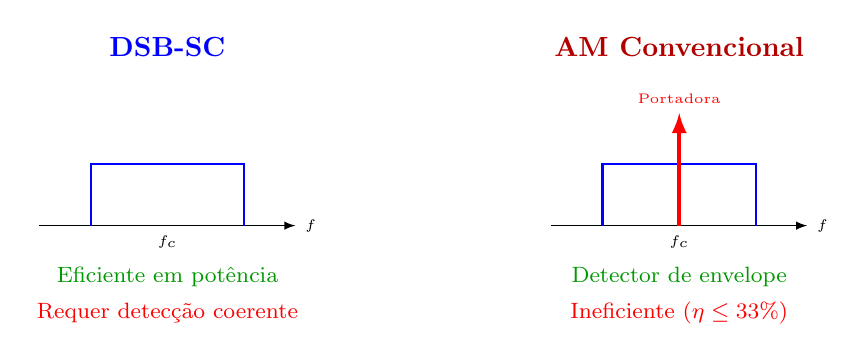
\begin{tikzpicture}[>=latex, scale=0.65]
% DSB-SC lado
\begin{scope}[xshift=-5cm]
\node[font=\normalsize\bfseries, blue] at (2,3.5) {DSB-SC};
\draw[->] (-0.5,0) -- (4.5,0) node[right, font=\tiny] {$f$};
\draw[thick, blue] (0.5,0) -- (0.5,1.2) -- (3.5,1.2) -- (3.5,0);
\node[below, font=\tiny] at (2,0) {$f_c$};
\node[font=\footnotesize, green!60!black] at (2,-1) {Eficiente em potência};
\node[font=\footnotesize, red] at (2,-1.7) {Requer detecção coerente};
\end{scope}
% AM Convencional lado
\begin{scope}[xshift=5cm]
\node[font=\normalsize\bfseries, red!70!black] at (2,3.5) {AM Convencional};
\draw[->] (-0.5,0) -- (4.5,0) node[right, font=\tiny] {$f$};
\draw[thick, blue] (0.5,0) -- (0.5,1.2) -- (3.5,1.2) -- (3.5,0);
\draw[thick, red, ->, line width=1.5pt] (2,0) -- (2,2.2);
\node[above, font=\tiny, red] at (2,2.2) {Portadora};
\node[below, font=\tiny] at (2,0) {$f_c$};
\node[font=\footnotesize, green!60!black] at (2,-1) {Detector de envelope};
\node[font=\footnotesize, red] at (2,-1.7) {Ineficiente ($\eta \leq 33\%$)};
\end{scope}
\end{tikzpicture}
\end{center}

\vspace{-0.2cm}

\begin{itemize}\setlength{\itemsep}{0pt}
\item \textbf{DSB-SC:} eficiente, mas receptor complexo
\item \textbf{AM Conv.:} receptor simples, mas desperdiça potência
\end{itemize}

\end{frame}

% %%%%%%%%%%%%%%%%%%%%%%%%%%%%%%%%%%%%%%%%%%%%
% EXERCÍCIOS — AM Convencional
% %%%%%%%%%%%%%%%%%%%%%%%%%%%%%%%%%%%%%%%%%%%%

\subsection*{Exercícios: AM Convencional}

% ============================================
\begin{frame}{Exercício AM Conv 1: Índice e Eficiência}

\only<1>{
Uma estação AM broadcast: $A_c = 50\,\text{V}$,
$f_c = 1200\,\text{kHz}$, $m(t) = \cos(2\pi \cdot 5000\, t)$, $\mu = 0.6$.

\vspace{0.2cm}

\begin{enumerate}[a)]
\item Escreva $s(t)$ e identifique portadora, LSB e USB.
\item Calcule $P_c$, $P_{sb}$ e $P_s$.
\item Calcule a eficiência $\eta$.
\item Se $\mu$ subir para 1.0, qual a nova eficiência?
\end{enumerate}
}

\only<2>{
\textbf{a)} $s(t) = 50[1 + 0.6\cos(2\pi\!\cdot\!5000\,t)]\cos(2\pi\!\cdot\!1.2\!\times\!10^6 t)$

Portadora: 1200 kHz, LSB: 1195 kHz, USB: 1205 kHz

\textbf{b)}
$P_c = \frac{50^2}{2} = 1250\,\text{W}$, \
$P_{sb} = \frac{0.36}{2}\cdot 1250 = 225\,\text{W}$, \
$P_s = \boxed{1475\,\text{W}}$

\textbf{c)} $\eta = \frac{225}{1475} = \boxed{15.3\%}$ \quad (84.7\% desperdiçado na portadora!)

\textbf{d)} $\mu = 1$: $\eta = \frac{1}{3} = \boxed{33.3\%}$ \quad (dobra, mas ainda 2/3 é portadora)
}

\end{frame}

% ============================================
\begin{frame}{Exercício AM Conv 2: Link Budget}

\only<1>{
Estação AM broadcast:

\begin{center}\small
\begin{tabular}{l l}
$P_{TX} = 10\,\text{kW}$, $\mu = 0.8$ & $f_c = 1\,\text{MHz}$ \\
$G_{TX} = 3\,\text{dBi}$ & $G_{RX} = 0\,\text{dBi}$ \\
$d = 50\,\text{km}$ & $P_{\min} = -90\,\text{dBm}$ \\
\end{tabular}
\end{center}

\begin{enumerate}[a)]
\item Calcule a perda de espaço livre (FSPL).
\item Qual a potência recebida $P_{RX}$?
\item Qual a margem do link?
\item Compare: se fosse DSB-SC com mesma $P_{TX}$, mudaria algo no link budget?
\end{enumerate}
}

\only<2>{
\textbf{a) FSPL} ($\lambda = 300\,\text{m}$):
$\text{FSPL} = 20\log_{10}\!\left(\frac{4\pi \times 50000}{300}\right) = \boxed{84.4\,\text{dB}}$

\textbf{b)} $P_{RX} = 70 + 3 - 84.4 + 0 = \boxed{-11.4\,\text{dBm}}$

\textbf{c)} Margem $= -11.4 - (-90) = \boxed{78.6\,\text{dB}}$ \quad (confortável!)

\textbf{d)} DSB-SC: mesmo $P_{TX}$ e FSPL $\rightarrow$ mesmo $P_{RX}$

Mas a potência \textbf{útil} muda: AM Conv usa 24\% para info, DSB-SC usa 100\%

Na prática, o detector de envelope do AM Conv é mais tolerante a ruído que o coerente do DSB-SC neste cenário
}

\end{frame}

% ============================================
\begin{frame}{Exercício AM Conv 3: Banda Básica e Banda Passante}

\only<1>{
Sinal de voz telefônica: $m(t)$ ocupa $300\,\text{Hz}$ a $3400\,\text{Hz}$.

\vspace{0.2cm}

\begin{enumerate}[a)]
\item Qual a largura de banda em banda básica?
\item Se modulado em AM convencional com $f_c = 100\,\text{kHz}$ e $\mu = 0.7$,
      qual a faixa em banda passante?
\item Qual a eficiência $\eta$?
\item Receptor super-heteródino com IF $= 455\,\text{kHz}$:
      qual a frequência do oscilador local?
\end{enumerate}
}

\only<2>{
\textbf{a)} $B_{\text{bb}} = 3400 - 300 = \boxed{3.1\,\text{kHz}}$

\textbf{b)} LSB: 96.6--99.7 kHz, USB: 100.3--103.4 kHz, Portadora: 100 kHz

$B_{\text{RF}} = 2 \times 3.4 = \boxed{6.8\,\text{kHz}}$

\textbf{c)} $\eta = \frac{0.49}{2.49} = \boxed{19.7\%}$

\textbf{d)} $f_{LO} = f_c + f_{IF} = 100 + 455 = \boxed{555\,\text{kHz}}$

\begin{center}
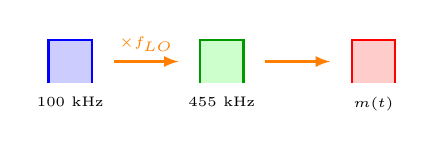
\begin{tikzpicture}[>=latex, scale=0.55]
\fill[blue!20] (0.5,0) -- (0.5,1) -- (1.5,1) -- (1.5,0) -- cycle;
\draw[thick, blue] (0.5,0) -- (0.5,1) -- (1.5,1) -- (1.5,0);
\node[below, font=\tiny] at (1,-0.1) {100 kHz};
\draw[->, thick, orange] (2,0.5) -- (3.5,0.5) node[midway, above, font=\tiny] {$\times f_{LO}$};
\fill[green!20] (4,0) -- (4,1) -- (5,1) -- (5,0) -- cycle;
\draw[thick, green!60!black] (4,0) -- (4,1) -- (5,1) -- (5,0);
\node[below, font=\tiny] at (4.5,-0.1) {455 kHz};
\draw[->, thick, orange] (5.5,0.5) -- (7,0.5);
\fill[red!20] (7.5,0) -- (7.5,1) -- (8.5,1) -- (8.5,0) -- cycle;
\draw[thick, red] (7.5,0) -- (7.5,1) -- (8.5,1) -- (8.5,0);
\node[below, font=\tiny] at (8,-0.1) {$m(t)$};
\end{tikzpicture}
\end{center}

Freq.\ imagem: $555 + 455 = 1010\,\text{kHz}$ (deve ser rejeitada!)
}

\end{frame}

% ============================================

